% @Author: Taha Bouhsine


%%%%%%%%%%%%%%%%%%%%%%%%%%%%
% CHAPTER                  %
%%%%%%%%%%%%%%%%%%%%%%%%%%%%
\setcounter{mtc}{7}
\chapter{Project General Context }%
\label{chap:chapter_one}
\minitoc
%%%%%%%%%%%%%%%%%%%%%%%%%%%%
% SECTION                  %
%%%%%%%%%%%%%%%%%%%%%%%%%%%%
\section{ Project Presentation }
\subsection{Presentation}
\subsection{Problem}
For the last few years, all over the world crowdfunding become one of the main tools and funding source for most of the new startups and creative minds all over the globe,
so we sought to create a new crowdfunding application, that will bring and adopt all the creative minds and ambitious souls and provides them with a tool to seek funds from a global community,
and help people to back and fund the creator in their journey and help him showcase the ideas that will be brought to life through the direct support of others.
so the creators will be able to coordinate multiple campaigns easier, and will be able to find people who are willing to invest with little equity involved.
And we sought also to provide a platform that will allow for gatekeeping that will monitor and create symbiotic relations with other algorithms and information online by using cloud-based solutions for better access.
our platform can help leap the hurdle of lack of experience in each field. Letting the barrier of entry be lessened for everyone who has a dream.
\paragraph*{}
"Ideas are cheap, Execution is expensive" Even if you create a beautiful application with a beautiful User Interface, if you neglect even one aspect of the main functionalities, and built it with a half effort, you might result in a product that won't live for long, or if you were to use the wrong technologies for the project, you might as well find yourself limited and won't be able to create and bring the most out of your Idea.
\paragraph*{}
So for our project, there is a real challenge in creating a product that competes with all the other platforms out there,
and first of all, we have to define what are the objectives we are seeking to complete to get to that final product,
so one main thing we needed to get our self doing is to look for the philosophies of crowdfunding, and try to understand humans motivation that make them want to fund and help another human, and what makes the creator seek funds from this type of fund seeking,
so we read some articles that have studied and handled the academic side of crowdfunding, from the university of  researchers create [\cite{inproceedings}], which helped us in a great deal to understand the depth of our problem, and guided us into creating our application design, as some researchers whom are studying the psychology of giving seek to understand why certain people give and how to get more individuals to give.They suggest that goals, schema, information processing, memory, involvement, attitudes, affective processing, atmospherics, and consumer attributions and choices are the key elements of consumer behavior that drive the consumer decision process.
And that Creators are motivated to use crowdfunding platforms because it provides an easy, efficient, organized way to solicit and collect financial support from many people in a distributed network [\cite{crowdMotiv}]. By using web-based technologies, such as online payment systems and social media, creators are able to market and solicit resources safely and easily through crowdfunding platforms.
Funders motivations to Crowdfunding:
\begin{enumerate}
      \item Seek Rewards
      \item Help Others
      \item Support Creators and Causes
      \item Engage and Contribute to a Trusting and Creative Community
\end{enumerate}

Funders deterrents to Crowdfunding:
\begin{enumerate}
      \item Distrust of Creators’ Use of Funds
\end{enumerate}

One motivation of supporters in crowdfund-ing communities is the desire to collect external rewards such as an acknowledgment, a tangible artifact, or an experience. An acknowledgment may come in the form of a telephone call, while a tangible artifact may be a CD or gadget. An experience may involve, for instance, meeting with the creator. The creator’s goal is to provide rewards that satisfy the supporters’ desire to collect.

Creators motivations to Crowdfunding:
\begin{enumerate}
      \item Raise Funds
      \item Establish Relationships and form Connections
      \item Maintain Control
      \item Learn New Fundraising Skills
      \item Receive Validation and approval
      \item Replicate Successful Experience of Others
      \item Expands Awareness  of Work  through Social Media
\end{enumerate}

Creators deterrents to Crowdfunding:
\begin{enumerate}
      \item Inability to Attract Supporters
      \item Fear of Public Failure and Exposure
      \item Time and Resource Commitment
\end{enumerate}

Next up we will look at the main qualities and objectives we have to respect to create a great product.
\subsection{Objectives}

So one of our main objectives is to create a platform that can improve our user's experience and boost the chance of our creators to reach the maximum of the audience as well as facilitate the access and the funding process for our funders, and provide a place where they can build there trust and look for promising talents and empowering entrepreneurs to help in creating new possibilities.\\
And to do that we should focus on respecting the following objectives and take them in mind while designing and developing our platform.
\begin{enumerate}
      \item
            User Experience
            Making sure that our crowdfunding software solutions are easy to navigate for the end-user is a crucial part of the development process. If our customers are befuddled by how to navigate our application, then it is highly likely that they will leave and find another crowdfunding platform. Not only will we want a functional interface, but one that is eye-catching as well.
            One thing to take note of is the importance of giving them the terms and conditions within the first few steps, so they fully understand what to expect. This shows a dedication to transparency that many startups and entrepreneurs will appreciate.

      \item
            Account Management
            Our customers will want to know what is going on, and making it easy on them will help make our platform successful. That means setting up systems that make it very clear what’s going on with their project. We will want them to be able to access who has been investing, how much money they have, how far they are from their goal, and any other metric they need to run a successful campaign. This could also include reports for recharges, withdrawals all available via a simple to navigate dashboard.
      \item

            Report Generation
            As the platform owner, you need a way to benefit from your time spent on creating this site that will help so many people. So, ensuring you also have access to backed reports like rewards, investors, and such can help you help them, as they say. This means creating a dashboard that, just like for the actual campaign creators, is easy to navigate and gives you access to reports you can use to course-correct and upgrade the systems.
      \item
            Payment Gateway \& Marketing
            When starting a crowdfunding platform you will want to set it up with access to the right payment gateways. Each gateway has its features, and so doing some in-depth research into them will allow you to choose one or several that works for the largest number of potential customers.
\end{enumerate}


\section{Functionality}
The platforms operate by allowing those seeking finance to make a pitch on the site outlining how much money they need, what they need the money for, if anything, you get in return for contributing. Potential funders can then view pitches on the platform, interact with both those looking for finance and other potential funders and then decide whether or not they want to back the campaign. The majority of platforms operate the all–or–nothing model where, if the target amount is not raised within a given timeframe, contributions are returned to funders and no financing goes ahead, but we are using the Keep It All model, anything you raise is yours.

% TODO 
\section{Relevance}
Sahem is a unique crowdfunding app built primarily in MEAN Stack technologies. It has one type of user that can be two types at the same time: can be either a creator or a funder. A funder donates while a creator acquires the fund. This app has a trust-building mechanism called corroboration where funders can certify creators and allow creators to certify their claims through uploading documentary proofs in an image format. The final mode of crowdfunding takes place through the exchange of transactional information where Funders can pay and amount of monetary by a bank transfer or by card.
We took the chance in providing easy accessibility to the main functionalities of the platform, as we tried to ask what is the most thing that a user wants to do, and we tried to optimize the number of clicks that a user would have to make in order to do the actions he wants, so we sought to make both of the creation of a fundraiser, and funding a project accessible by a maximum of 3 clicks and after the creator starts a fundraiser he can directly share a link that can lead to the funding page, bypassing the project description and content, to help in making the funders fund in a very short time, instead of filling unnecessary forms and passing by multiple pages.
\section{Feasibility}
This project is technically and financially feasible. I will spend approximately nothing to host the app, and in the future, there is an option to pay as you grow, by generating income from cutting a \% from the funds at the end of each fundraiser, we will get the costs covered. With regards to the technical feasibility, it will be built in well-established MEAN Stack technologies, that have a low cost with great scalability, and maintainability.

Sahem is needed to connect people in the world. I believe if this product is marketed correctly many people will find the opportunity to innovate and create more projects that will raise funds easily because Sahem provides the following unique features:
\begin{enumerate}
      \item
            Trust-building through corroboration mechanism.
      \item
            Opportunity for long term commitment between Creators and Funders.
      \item
            Uses secure technologies on both the frontend and the backend, and any requests sent by the users are passed by multiple middlewares on the backend.
      \item
            Easy Navigation through simple user interface design built using Angular, a framework that helps in creating fast and reliable Single Page Applications.
      \item
            A headless backend, which allow us to create different frontend application afterward, and that are linked to the same backend.
      \item
            Global crowdfunding interaction, no limits between countries, everyone can fund or create fundraisers.
      \item
            Statistical analysis of need vis-à-vis people.
\end{enumerate}
\section*{ Project management }
Process-driven software development is based on rigorously defined activities and tasks that are also repeatable and measurable. Formal processes facilitate planning, analysis of requirements from multiple angles, design of high-quality software models by following standards and using team-based tools, and incorporation of quality through walkthroughs, inspections, and testing.
As a result, such formal processes enhance quality and maximize user benefits.
\subsection*{ Project Development Process }
The process of discipline is complex. This is because a process considers myriad different hard and soft factors that impact development. Many software developers argue that processes restrict their creativity. Far from that, processes enable creativity with value. This is because processes ensure the effort made by architects, designers, developers, and testers will be well directed toward the commonly agreed goals (business objectives) of a project. Processes also facilitate measures and metrics that indicate individual and team productivity and quality. Metrics and measurements in software projects also enable the assignment of responsibilities and accountabilities.
\paragraph*{}
The iterations and increments shown in Figure 4.4 are the basis of most modern-day approaches to developing good software. In this iterative and incremental approach, no deliverable is produced in a single attempt. Instead, at least three iterations (repetitions) are undertaken before producing a deliverable.
This is followed by incrementally adding another package, which would have its own three or more iterations. The three terms iteration, incremental, and parallel are further discussed next.
\begin{figure}[!ht]
      \center
      \includegraphics[scale=0.40]{assets/iteration.png}
      \caption{Iterative process project life cycle}
      \label{fig:iterationlifecycle}
\end{figure}
\paragraph*{Iterative}
The iterative aspect of a process enables the repetition of tasks. As a result, the deliverables are produced gradually. For example, when a use case is iterated, additional material is added to the description of the use case—such as alternative flows within the use case. The iterative approach encourages a slow and steady philosophy rather than hurrying and finishing up a deliverable in the first attempt.
Deliverables are gradually matured by undertaking at least three iterations across multiple other deliverables. For example, while following an iterative process one might move from an initial use case to another use case in another diagram, then identify classes and draw a sequence diagram before coming back to the original use case and completing it.
\paragraph*{Incremental}
The incremental aspect of a process enables adding new elements and diagrams to an existing deliverable. An example is to add new packages to existing or developing packages. New requirements are thus discovered and modeled incrementally. This incremental aspect of the process enables the creation of parts of a system in as complete a manner as possible before proceeding with the development of additional parts of the system. The incremental aspect of a process often goes hand in hand with the iterative aspect. For example, while a new deliverable is incrementally added (a new use case), an existing deliverable is iteratively augmented during a later iteration (e.g., additional steps added to a use case).
\clearpage
\subsection*{Monitoring and planning}
\subsubsection*{Monitoring}
Breaking down a project into subparts to enable controlled execution and monitoring of the project.\\
Figure \ref{fig:bos} shows how the business objective is divided into subparts. to arrive at acceptable performance criteria of the system, the BO gets further divided into smaller parts or subject areas.
\begin{figure}[!ht]
      \center
      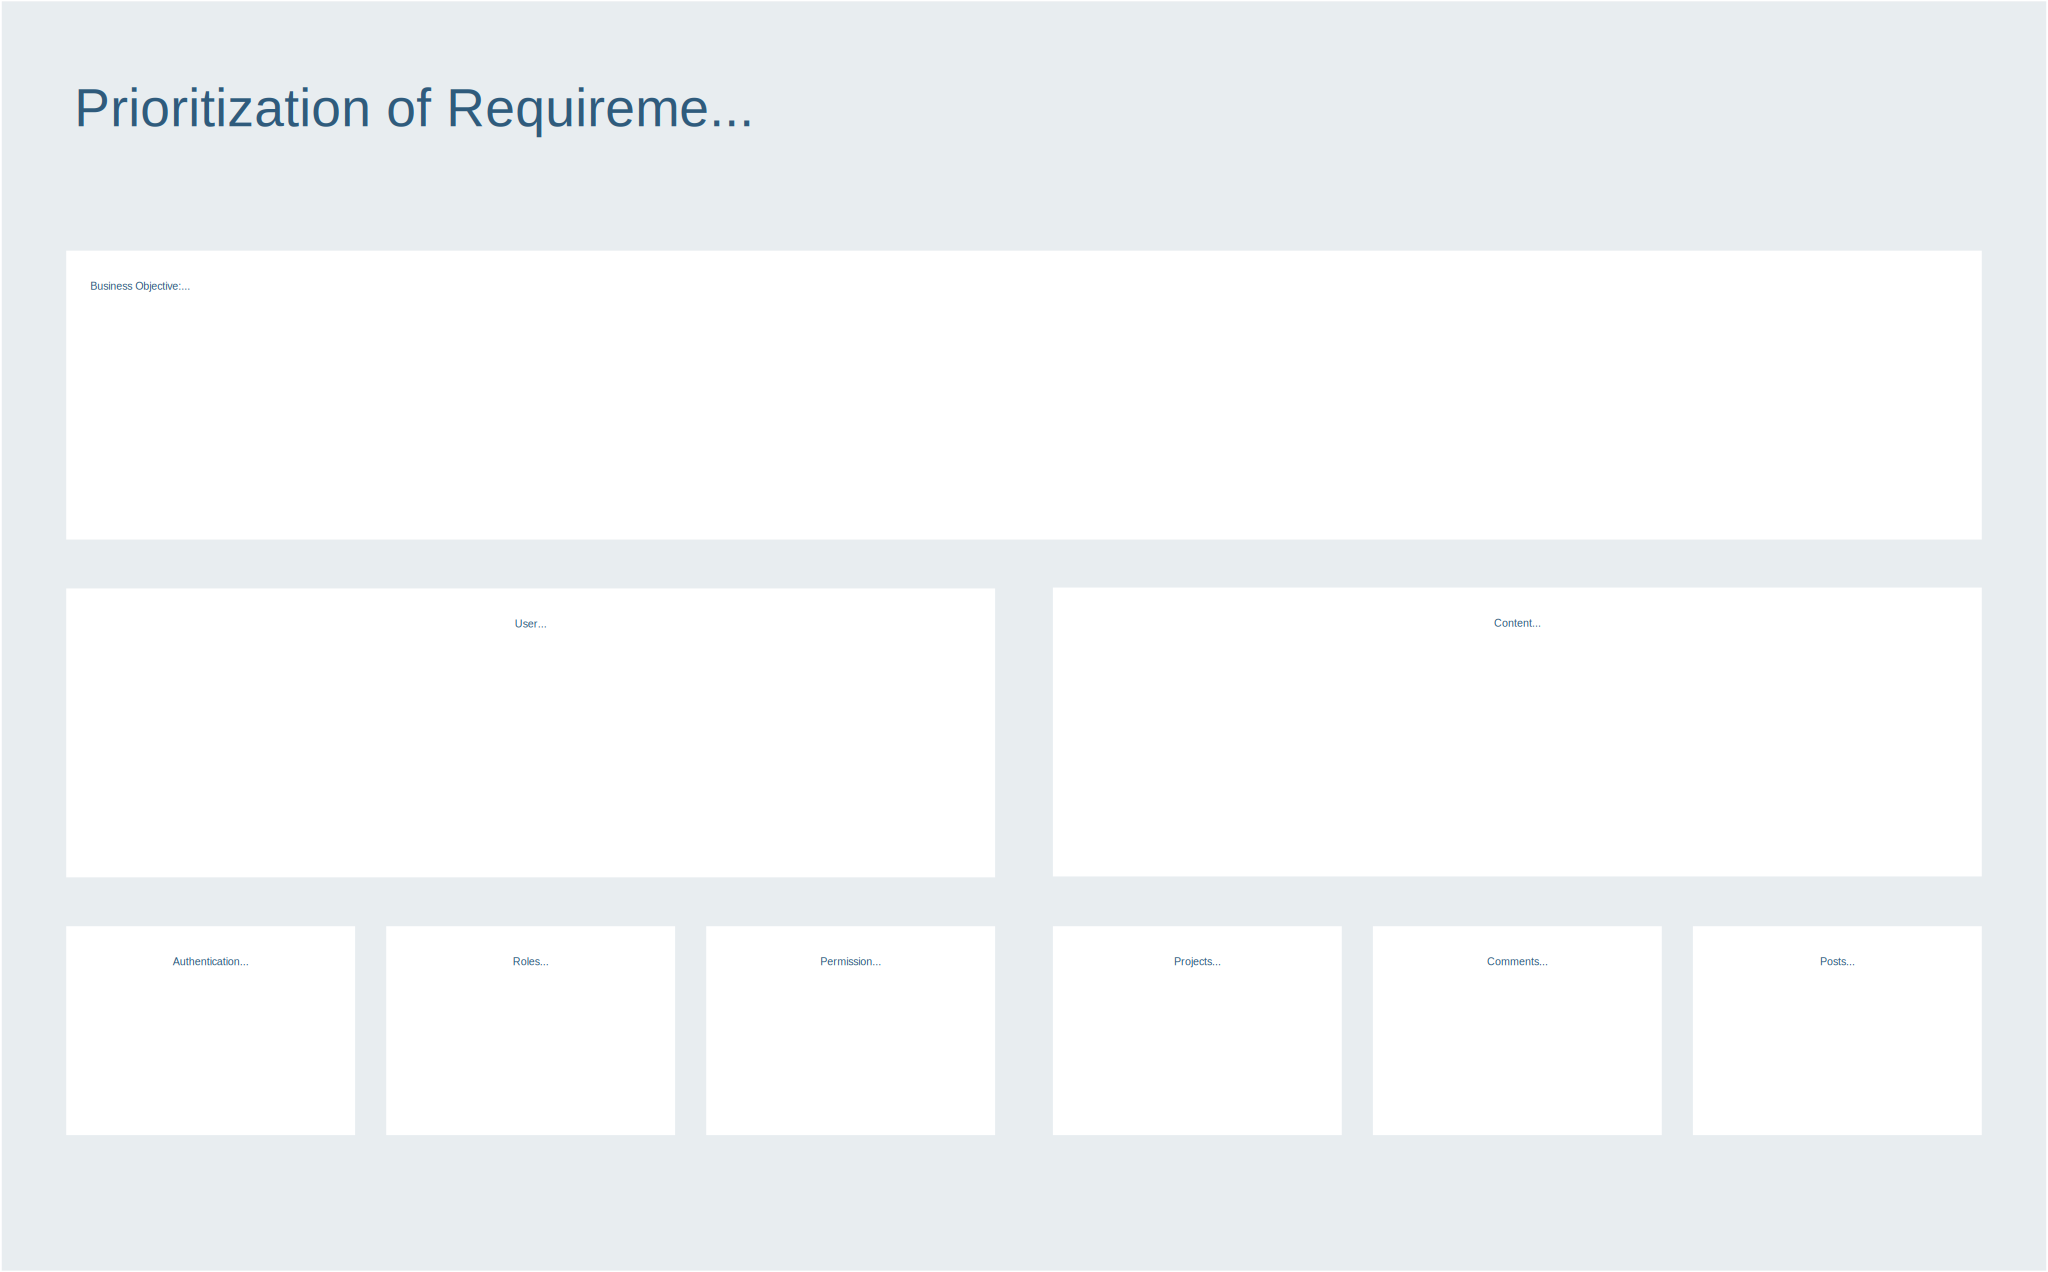
\includegraphics[scale=0.20]{assets/bos.png}
      \caption{Iterative process project life cycle}
      \label{fig:bos}
\end{figure}
\subsubsection*{Planning}
Provide precise routing of one or more business processes with opportunities to optimize on time and costs associated with the processes.
\includepdf[pages=-,angle=90,]{assets/ganttchart.pdf}
